\subsection{BlissBook}
\begin{figure}[h]
	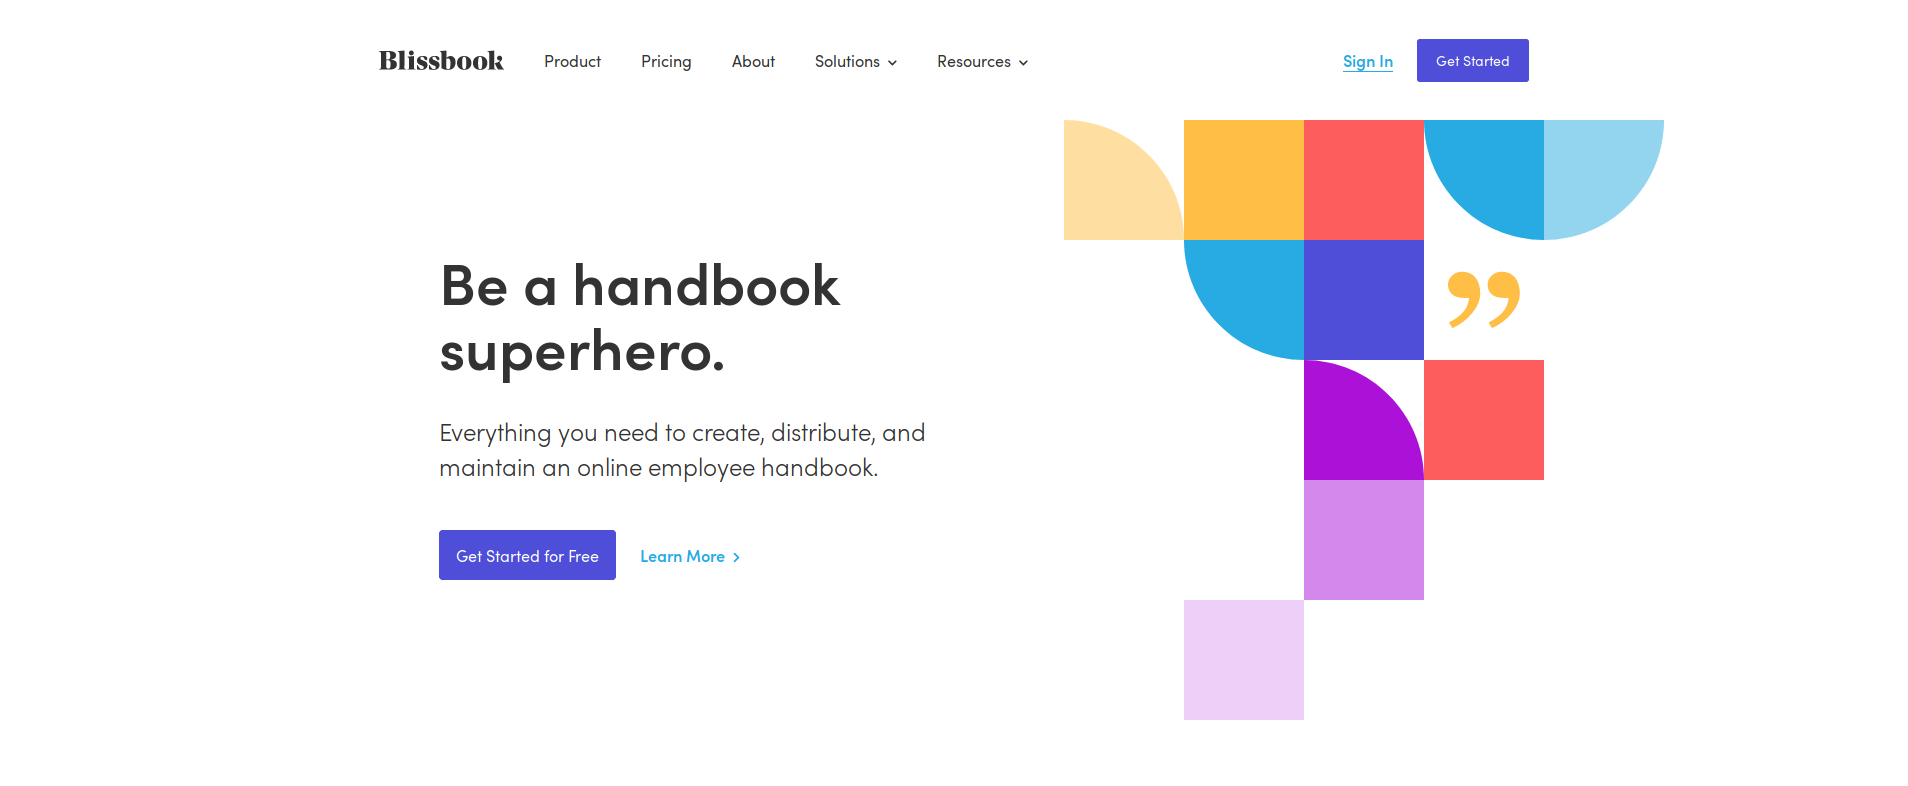
\includegraphics[width=1\textwidth]{billeder/BlissBooks.png}
	\caption{BlissBook landing page}
\end{figure}
BlissBook is a \textit{Software as a Service} (SaaS) employee handbook system, developed by the company of the same name starting in 2013. % cite https://blissbook.com/about
This chapter is mostly based upon information from their website


BlissBook based on a rich text editor which supports collabrative editing, and has features such as access control, digital signatures to keep track of which employees have read which handbooks, and sending notifications to employees when new versions are released.

They offer 99.9\% uptime.

They offer exports of all data on the platform, even after the account is closed.

On the security front, the BlissBook website does not mention any certificatations on their software, besides them offering AES-256 encryption. % https://blissbook.com/information-security
